\documentclass[compress]{beamer}

\mode<presentation>
{
  %\usetheme{Warsaw}
  %\usecolortheme{spruce}
  % or ...
	%\useoutertheme{infolines}
  %\setbeamercovered{transparent}
  
  \usetheme{CambridgeUS}
    \setbeamercolor{item projected}{bg=darkred}
    \setbeamertemplate{enumerate items}[default]
    \setbeamertemplate{navigation symbols}{}
    \setbeamercovered{invisible}
    \setbeamercolor{block title}{fg=darkred}
    \setbeamercolor{local structure}{fg=darkred}
  
  % or whatever (possibly just delete it)
}

\usepackage{verbatim} 
\usepackage{listings}
\usepackage{tikz}
\usetikzlibrary{arrows}
\usetikzlibrary{shapes}
\tikzstyle{block}=[draw opacity=0.7,line width=1.4cm]

\newcommand{\bigpause}{\bigskip \pause}

\lstloadlanguages{C++}
\lstnewenvironment{code}
	{%\lstset{	numbers=none, frame=lines, basicstyle=\small\ttfamily, }%
	 \csname lst@SetFirstLabel\endcsname}
	{\csname lst@SaveFirstLabel\endcsname}
\lstset{% general command to set parameter(s)
	language=C++, basicstyle=\footnotesize\sffamily, keywordstyle=\slshape,
	emph=[1]{tipo,usa}, emphstyle={[1]\sffamily\bfseries},
	basewidth={0.47em,0.40em},
	columns=fixed, fontadjust, resetmargins, xrightmargin=5pt, xleftmargin=15pt,
	flexiblecolumns=false, tabsize=2, breaklines,	breakatwhitespace=false, extendedchars=true,
	numbers=left, numberstyle=\tiny, stepnumber=1, numbersep=9pt,
	frame=l, framesep=3pt,
}

\usepackage[spanish]{babel}
% or whatever

\usepackage[utf8]{inputenc}
% or whatever

\usepackage{times}
\usepackage[T1]{fontenc}
% Or whatever. Note that the encoding and the font should match. If T1
% does not look nice, try deleting the line with the fontenc.


\title[Modelado con grafos] % (optional, use only with long paper titles)
{Modelado con grafos}

\author[Melanie Sclar] % (optional, use only with lots of authors)
{~Melanie Sclar}
% - Give the names in the same order as the appear in the paper.
% - Use the \inst{?} command only if the authors have different
%   affiliation.
\institute[UBA] % (optional, but mostly needed)
{
  %\inst{1}%
  Facultad de Ciencias Exactas y Naturales\\
  Universidad de Buenos Aires
}
%\date[TC 2014] % (optional, should be abbreviation of conference name)
%{Training Camp 2014}

% Ac¿ se puede insertar el logo de la UBA
% \pgfdeclareimage[height=0.5cm]{university-logo}{university-logo-filename}
% \logo{\pgfuseimage{university-logo}}



% Delete this, if you do not want the table of contents to pop up at
% the beginning of each subsection:
\AtBeginSubsection[]
{
  \begin{frame}<beamer>{Contenidos}
    \tableofcontents[currentsection,currentsubsection]
  \end{frame}
}

\newcommand{\be}{\begin{equation*}}
\newcommand{\ee}{\end{equation*}}
\newcommand{\state}[1]{\left|\,#1\,\right\rangle}
\newcommand{\costate}[1]{\left\langle\,#1\,\right|}
\newcommand{\trace}{\text{Tr}}
\newcommand{\su}{\uparrow}
\newcommand{\sd}{\downarrow}
\newcommand{\im}{\text{Im}}
\newcommand{\re}{\text{Re}}

% If you wish to uncover everything in a step-wise fashion, uncomment
% the following command:

%\beamerdefaultoverlayspecification{<+->}


\begin{document}
\pgfdeclarelayer{background}
\pgfsetlayers{background,main}
\begin{frame}
  \titlepage
\end{frame}

\begin{frame}{Contenidos}
  \tableofcontents
  % You might wish to add the option [pausesections]
\end{frame}


\section{Representaci\'on de grafos}
\subsection{Matriz de adyacencia}
\begin{frame}{Matriz de adyacencia}
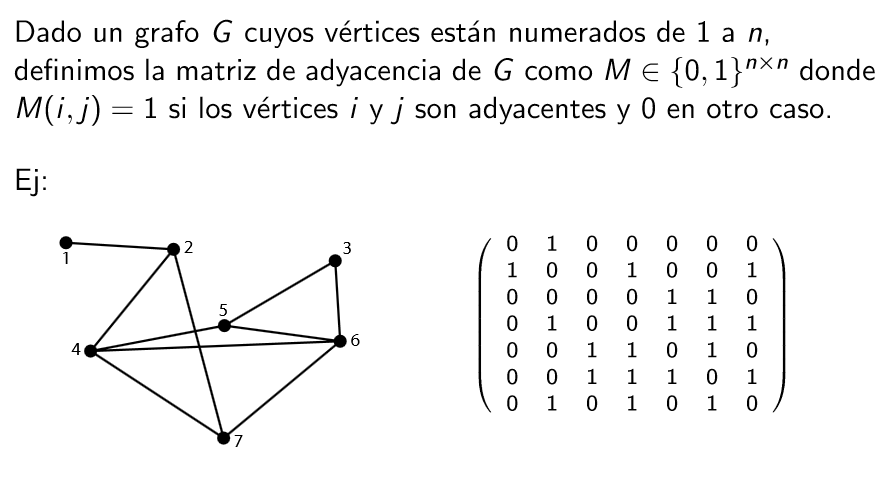
\includegraphics[scale=0.5]{matriz-adyacencia.png}
\end{frame}

\begin{frame}{Matriz de adyacencia}
Esta es una de las representaciones m\'as utilizadas. Si bien el ejemplo es para un grafo no dirigido, tambi\'en se puede utilizar la misma estructura para grafos dirigidos y grafos con pesos.
\bigskip

{\bf Ventajas}
\pause
\invisible<1> {
	\begin{itemize}
		\item Permite saber si existe o no arista entre dos nodos cualesquiera en O(1).
		\item Es muy f\'acil de implementar, $matrizAdy[i][j]$ guarda toda la informaci\'on sobre la arista.
	\end{itemize}
}
\bigpause
{\bf Desventajas}
\pause
\invisible<1> {
	\begin{itemize}
		\item La complejidad espacial: se necesitan $n^2$ casillas para representar un grafo de $n$ nodos.
	\end{itemize}
}
\end{frame}



\subsection{Lista de adyacencia (o listas de vecinos)}

\begin{frame}{Lista de adyacencia}
Coloquialmente la llamamos {\it lista de vecinos} pues para cada nodo guardamos la lista de nodos para los que existe una arista que los conecta (o sea, los vecinos).
\bigskip
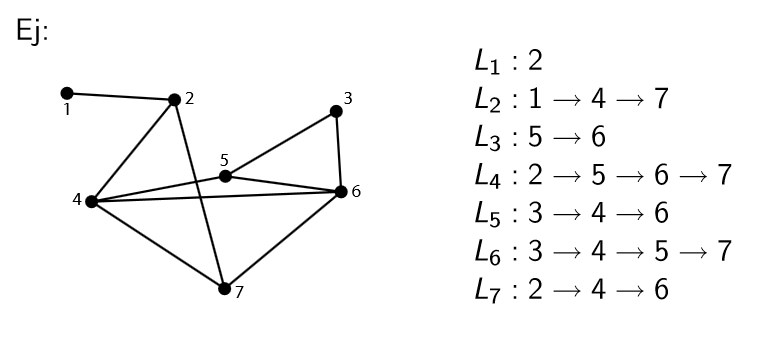
\includegraphics[scale=0.5]{lista-vecinos.png}
\end{frame}

\begin{frame}{Lista de adyacencia}
Nuevamente, con la misma idea tambi\'en se pueden modelar grafos dirigidos y con pesos.\bigskip

En principio, la lista de vecinos no tiene por qu\'e estar ordenada. Pero asumiendo que s\'i lo est\'a, ?`Qu\'e complejidad ser\'a necesaria para consultar si dos nodos tienen una arista que los une? \pause {\bf O(lg n)} \bigpause

La complejidad espacial de esta representaci\'on ser\'a posiblemente mucho menor. ?`Cu\'anta memoria necesitaremos para un grafo de $n$ nodos y $m$ aristas? \pause {\bf O(m+n)}
\end{frame}

\subsection{Lista de incidencia (o lista de aristas)}
\begin{frame}{Lista de incidencia}
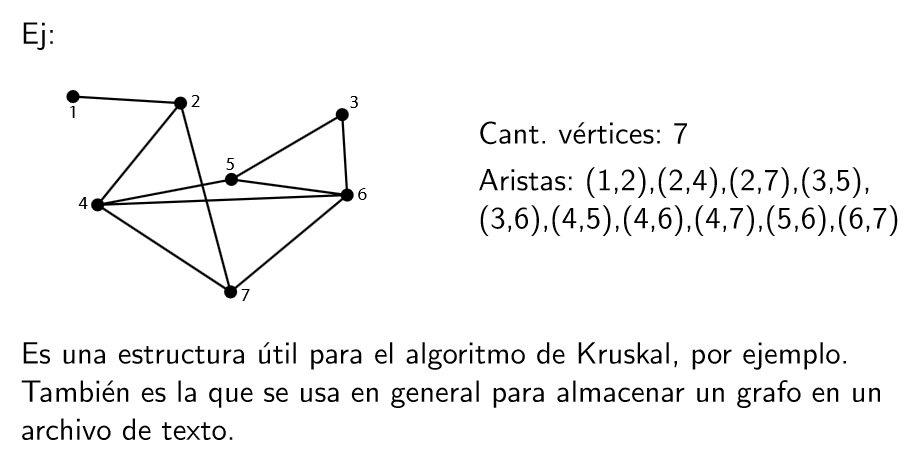
\includegraphics[scale=0.5]{lista-aristas.png}
\end{frame}

\section{Problemas con grafos}
\subsection{Calentando motores}
\begin{frame}{Problema sencillo para empezar}
En una ciudad con forma de grilla hay $h$ calles horizontales y $v$ calles verticales. Adem\'as, algunas esquinas est\'an obstaculizadas por diversos motivos, y no se puede pasar por all\'i.\bigskip

Queremos partir desde nuestra casa y llegar a la facultad. ?`Ser\'a posible lograrlo? \\ Dise\~nemos un algoritmo eficiente para resolver este problema. \bigskip

{\bf Pista:} el problema se puede resolver con complejidad temporal $O(v h)$

\end{frame}

\subsection{Modelar un problema con un grafo no trivial}
\begin{frame}{Modelar un problema con un grafo no trivial}
Muchas veces, modelar un problema con el grafo que el enunciado casi expl\'icitamente nos describe no es suficiente para cumplir con los requerimientos de eficiencia que se nos piden (o a veces, ni siquiera sabr\'iamos c\'omo resolverlo con ese grafo que nos dan).\bigskip

Para eso, durante la clase de hoy intentaremos {\bf pensar en grafos un poco m\'as ricos de los que venimos viendo, con m\'as par\'ametros}, que nos permitan resolver los problemas eficientemente. \bigskip

Como suele suceder, esto es un trade-off: {\bf al ganar en complejidad temporal, podemos perder en complejidad espacial}.
\end{frame}

\subsection{En la altura, la bici no dobla}
\begin{frame}{En la altura, la bici no dobla}
Melanie vive en la ciudad que mencionamos anteriormente: tiene forma de grilla, con $h$ calles horizontales y $v$ calles verticales. Adem\'as, algunas esquinas est\'an obstaculizadas por diversos motivos, y no puede pasar por all\'i.\bigskip

Recientemente Melanie se compr\'o una bicicleta y ya aprendi\'o a andar sin rueditas, pero doblar todav\'ia le cuesta. Le gustar\'ia poder ir en bici de su casa a la facultad minimizando la cantidad de veces que tiene que doblar en una esquina.
?`C\'omo la podemos ayudar? \bigskip
\end{frame}

\begin{frame}{Spoilers - idea 1}

Crear un grafo donde cada nodo describa una esquina y la direcci\'on de la que provenimos con la bici. As\'i, {\bf el nodo ser\'a una tupla (fila, columna, direcci\'on)}, y se conectar\'an dos nodos si y s\'olo si de un estado puedo pasar al otro. Adem\'as, si para pasar de un estado a otro debo doblar en una esquina, la arista tendr\'a costo 1. De lo contrario, tendr\'a costo 0.
\bigskip

Luego, tendremos un grafo con aristas de peso 0 \'o 1, y queremos saber cu\'al es el camino de costo m\'inimo desde la esquina inicial hasta la final. O(vh lg(vh)) si usamos Dijkstra con cola de prioridad.

\end{frame}


\begin{frame}{Spoilers - idea 2}

Ahora cada nodo adem\'as contendr\'a cu\'antos giros fue necesario realizar para llegar a cada esquina. As\'i, {\bf el nodo ser\'a una tupla (fila, columna, cantidad de giros usados hasta el momento, direcci\'on)}, y se conectar\'an dos nodos si y s\'olo si de un estado puedo pasar al otro.
\bigskip

Notar que este grafo no tendr\'a pesos, y lo que queremos preguntar es si ser\'a posible llegar a alg\'un nodo final cualquiera sea la cantidad de giros y la direcci\'on del mismo. Para ello ser\'a necesario recorrer el grafo (por ejemplo usando BFS) y ver si el nodo salida y alguna de las llegadas se encuentran en la misma componente conexa. Linealmente recorremos todos los posibles nodos llegada, y retornamos aquel cuya cantidad de giros necesarios sea m\'inima. \bigskip

\end{frame}

\begin{frame}{Spoilers - idea 2 (c\'alculo de complejidad)}

Llamemos $g$ a la cantidad m\'axima de giros posibles a realizar en el tablero.
As\'i, como BFS es lineal en el tama\~no de la entrada, y tenemos $v \times h \times g \times 2$ nodos en nuestro modelado (y cada nodo tiene grado a lo sumo 4), la recorrida del grafo ser\'a O(vhg).
\bigskip

Al final recorremos linealmente todos los posibles nodos finales, que como tienen fija la esquina en la que terminan son solamente $2g$ nodos. As\'i, la complejidad total del algoritmo es $O(vhg) + O(2g) = O(vhg)$
\end{frame}


\subsection{Prince of Persia}
\begin{frame}{Prince of Persia}
Mientras el sult\'an estaba luchando en una guerra en una tierra extranjera, su visir Jaffar, un brujo, tom\'o el poder por la fuerza. El deseo m\'as profundo de Jaffar es casarse con la hija del Sult\'an, pero ella ya tiene otro amor. Entonces, Jaffar la encerr\'o en una torre y le orden\'o que se case con \'el o de lo contrario la ejecutar\'a en $x$ minutos. \bigskip

Para asegurarse de que nadie la venga a salvar antes de que termine el tiempo, arroj\'o a su enamorado a una mazmorra con $n$ plataformas. Todas las plataformas tienen pinches que suben y bajan a un ritmo constante, pero posiblemente distintos entre s\'i. \bigskip
\end{frame}


\begin{frame}{Prince of Persia}
Originalmente el protagonista se encuentra en la plataforma $s$, y quiere llegar a la plataforma $e$ antes de que asesinen a su amada. Debe lograrlo saltando entre plataformas, y siempre teniendo cuidado de no morir al caer sobre pinches (o esperar demasiado tiempo y ser mortalmente atravesado). \bigskip

Adem\'as s\'olo puede moverse entre plataformas en minutos enteros, y las plataformas tambi\'en suben y bajan en minutos enteros.
?`Lo podr\'a lograr?
\end{frame}

\begin{frame}
\begin{center}
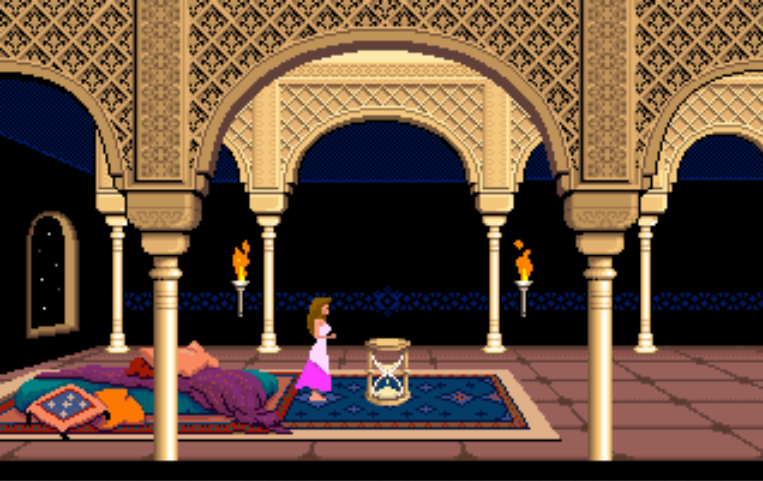
\includegraphics[scale=0.4]{prince-of-persia-waiting.png}

\bigskip

A pensar...
\end{center}
\end{frame}

\begin{frame}{Spoiler}
Es necesario notar que no es lo mismo estar en un nodo en un tiempo que en otro, pues a veces podr\'ia haber pinches y otras no. Es por eso que nuestros nodos ser\'an de la forma $(nodo, tiempo)$, y conectaremos dos nodos (a, t) y (b, t+1) si y s\'olo si a y b son vecinos (o $a=b$) y en $t+1$ no hay pinches en dicho nodo. \bigskip

Una vez armado ese grafo, notamos que nuestro nodo inicial es el (nodo\_inicial, 0), y queremos saber si es posible llegar a \\ (nodo\_final, y) con $y \leq x$. \\ Para ello, recorreremos el grafo con un BFS partiendo de (nodo\_inicial, 0) y veremos si existe alg\'un (nodo\_final, y) al que se pueda llegar (es decir, que est\'e en su misma componente conexa). \bigskip

Nuevamente, como el BFS es lineal en el tama\~no de la entrada y hay $n \times x$ nodos y a lo sumo $m \times x$ aristas, la complejidad ser\'a O(nx+mx).
\end{frame}
\end{document}